\section{设计}
\label{kvdirect:sec:architecture}

\subsection{系统架构}

KV-Direct使\textit {远程直接键值访问}成为可能。
客户端将\textit {KV-Direct 操作}(\S \ref {kvdirect:sec:kv-operations})发送到KVS服务器,而可编程网卡处理请求并发送回结果,绕过CPU。
KVS服务器上的可编程网卡是一个重新配置为\textit {KV处理器}的FPGA(\S \ref {kvdirect:sec:kv-processor})。
图\ref {kvdirect:fig:kvdirect-arch}显示了KV-Direct的架构。

\subsection{KV-Direct 操作}
\label{kvdirect:sec:kv-operations}

\begin{table}
\centering
\caption{KV-Direct 操作。}
\label{kvdirect:tab:kv-operations}

\small
\begin{tabular}{p{.4\textwidth}|p{.5\textwidth} }
\toprule
get ($k$) $\rightarrow v$ & Get the value of key $k$. \\
\midrule
put ($k, v$) $\rightarrow$ bool & Insert or replace a $(k, v)$ pair. \\
\midrule
delete ($k$) $\rightarrow$ bool & Delete key $k$. \\
\midrule
\midrule
update{\_}scalar2scalar ($k, \Delta, \lambda(v, \Delta) \rightarrow v$) $\rightarrow v$ & Atomically update the value of key~$k$ using function~$\lambda$ on scalar~$\Delta$, and return the original value. \\
\midrule
update{\_}scalar2vector ($k, \Delta, \lambda(v, \Delta) \rightarrow v$) $\rightarrow [v]$ & Atomically update all elements in vector~$k$ using function~$\lambda$ and scalar~$\Delta$, and return the original vector. \\
\midrule
update{\_}vector2vector ($k, [\Delta], \lambda(v, \Delta) \rightarrow v$) $\rightarrow [v]$ & Atomically update each element in vector~$k$ using function~$\lambda$ on the corresponding element in vector~$[\Delta]$, and return the original vector. \\
\midrule
reduce ($k, \Sigma, \lambda(v, \Sigma) \rightarrow \Sigma$) $\rightarrow \Sigma$ & Reduce vector~$k$ to a scalar using function~$\lambda$ on initial value, and return the reduction result~$\Sigma$. \\
\midrule
filter ($k, \lambda(v) \rightarrow$ bool) $\rightarrow [v]$ & Filter elements in a vector~$k$ by function~$\lambda$, and return the filtered vector. \\
\bottomrule
\end{tabular}

\end{table}

KV-Direct将单面RDMA操作扩展到键值操作,如表\ref {kvdirect:tab:kv-operations}中所述。
除了表\ref {kvdirect:tab:kv-operations}顶部所示的标准KVS操作外,KV-Direct还支持两种类型的向量运算:
将标量发送到服务器上的NIC,NIC将更新应用于向量中的每个元素;或者向服务器发送一个向量,并且NIC逐个元素地更新原始向量。
此外,KV-Direct支持用户定义的更新功能,作为原子操作的概括。
更新功能需要在执行前预先注册并编译为硬件逻辑。
使用用户定义的更新功能的KV操作类似于\textit {动态消息}(active messages)\cite {eicken1992active},从而节省了通信和同步成本。

当对键执行向量操作更新(update),归约(reduce)或过滤(filter)时,其值被视为固定位宽元素的数组。
每个函数 $\lambda$ 对向量中的一个元素,客户端指定的参数 $\Delta$ 和/或初始值 $\Sigma$ 进行归约操作。
KV-Direct开发工具链多次复制$\lambda$以利用FPGA中的并行性并将计算吞吐量与PCIe吞吐量相匹配,然后使用高级综合(HLS)工具将其编译为可重新配置的硬件逻辑\cite {aoc} 。
HLS工具自动提取复制函数中的数据依赖性,并生成完全流水线的可编程逻辑。
在执行KVS客户端之前,KVS服务器上的可编程NIC应加载包含展开的$\lambda$的硬件逻辑。

使用用户定义函数的更新操作能够对矢量值进行常规流处理。
例如,网络处理应用程序可以将该向量解释为用于网络功能的分组流\cite{li2016clicknp}或用于分组事务的一堆状态\cite {sivaraman2016packet}。
完全在可编程NIC中的单对象事务处理也是可能的,例如,在TPC-C基准中包围S\_QUANTITY \cite {council2010tpc}。
向量归约操作支持PageRank \cite {page1999pagerank}中的邻居权重累积。
可以使用向量过滤操作来获取稀疏向量中的非零值。

\subsection{KV 处理器}
\label{kvdirect:sec:kv-processor}

\begin{figure}[t]
\centering
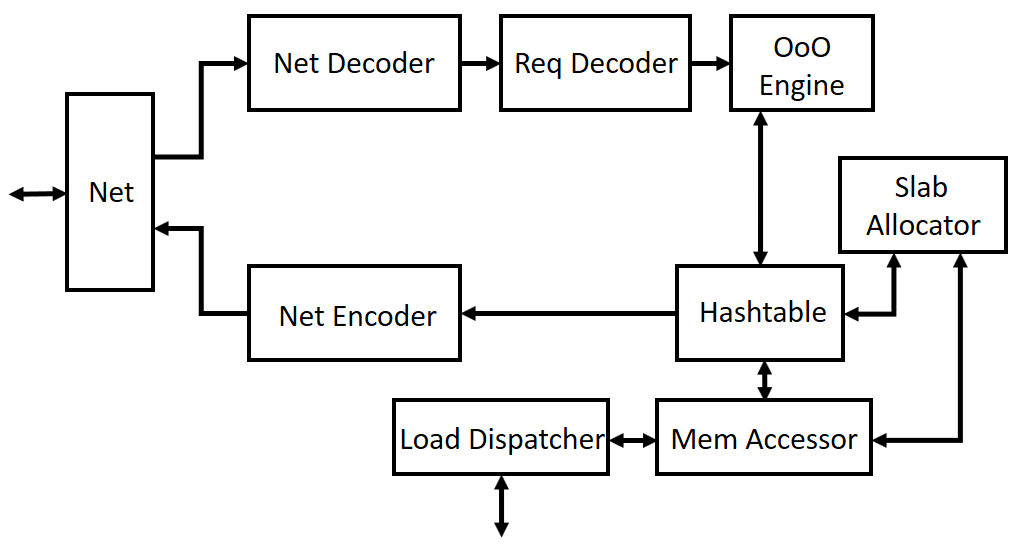
\includegraphics[width=0.6\textwidth,page=1]{processor_architecture.PNG}
\caption{KV 处理器架构。}
\label{kvdirect:fig:kvprocessor-arch}

\end{figure}

如图\ref {kvdirect:fig:kvprocessor-arch}所示,KV处理器从板载NIC接收数据包,解码向量操作并缓冲保留站中的KV操作(\S \ref {kvdirect:sec:ooo})。
接下来,乱序执行引擎(\S \ref {kvdirect:sec:ooo})从保留站向操作解码器发出独立的KV操作。
根据操作类型,KV处理器查找哈希表(\S \ref {kvdirect:sec:hashtable})并执行相应的操作。
为了最小化内存访问次数,较小的KV对在哈希表中内联(inline)存储,其他的KV对存储在slab内存分配器(\S \ref {kvdirect:sec:slab})的动态分配内存中。
散列索引和slab分配的内存都由统一的内存访问引擎(\S \ref {kvdirect:sec:dram-cache})管理,它通过PCIe DMA访问主机内存并缓存部分主机内存。板载DRAM。
在KV操作完成之后,结果被发送回无序执行引擎(\S \ref {kvdirect:sec:ooo})以在保留站中找到并执行匹配的KV操作。

正如\S \ref {kvdirect:sec:challenge}中所讨论的,PCIe操作吞吐量的稀缺性要求KV处理器在DMA访问上节俭。
对于GET操作,至少需要读取一次内存。
对于PUT或DELETE操作,对于哈希表,一次读取和一次写入最小。
基于日志的数据结构可以实现每个PUT一次写入,但它牺牲了GET性能。
KV-Direct仔细设计哈希表,以便在每次查找和插入时实现接近理想的DMA访问,以及内存分配器。每次动态内存分配平摊下来,只需不到0.1次DMA操作。

\subsubsection{哈希表}
\label{kvdirect:sec:hashtable}

\begin{figure}[t]
\centering
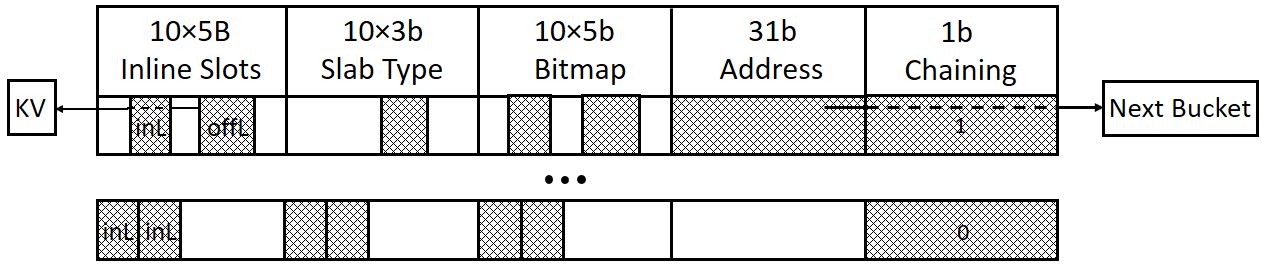
\includegraphics[width=1.0\textwidth,page=1]{hashline.PNG}
\caption{哈希索引结构。 每行是一个哈希桶,包含10个哈希槽,每个哈希槽3位板内存类型,一个位图标记内联KV对的开始和结束,以及指向哈希冲突下一个链接桶的指针。}
\label{kvdirect:fig:hashtable}

\end{figure}

为了存储可变大小的KV,KV存储分为两部分。 第一部分是哈希索引(图\ref {kvdirect:fig:hashtable}),它包含固定数量的\textit {哈希桶}。 每个哈希桶包含几个\textit {哈希槽}和一些元数据。 内存的其余部分是动态分配的,由slab分配器(\S \ref {kvdirect:sec:slab})管理。
初始化时配置的\textit {哈希索引比率}确定为哈希索引分配的内存百分比。
哈希索引比率的选择将在\S \ref {kvdirect:sec:hashtable-eval}中讨论。

%\textbf{Hash Table.}
%Each bucket includes 10 hash slots, 3b type code per slot, 50b metadata, plus 31b address and a valid bit of the next chained bucket, as shown in Figure~\ref{kvdirect:fig:hashtable}.
%For offline KVs, each hash slot needs to store 31b of address, 9b of secondary hash and 3b type code for the slab size.
%For inline KVs, to mark the begin and end of each hash slot, as well as the separation between inline key and value, the information is encoded in a 50b metadata corresponding to 50 bytes of hash slots.
%The inline keys and secondary hashes of offline keys in all hash slots are compared in parallel, and the first match is found.

每个散列槽包括指向动态分配的存储器中的KV数据的指针和辅助散列。
辅助哈希是一种启用并行内联检查的优化。始终检查密钥以确保正确性,但需要额外的一次内存访问。
假设主机内存中的64~GiB KV存储和32字节分配粒度(内部碎片和分配元数据开销之间的权衡),指针需要31位。
9位的二级散列给出1/512误报可能性。
累积地,散列槽大小是5个字节。
为了确定散列桶大小,我们需要在每个桶的散列槽数和DMA吞吐量之间进行权衡。
图\ref {kvdirect:fig:dma-tput}表明DMA读取吞吐量低于64B粒度受DMA引擎中PCIe延迟和并行性的约束。
由于哈希冲突的可能性增加,小于64B的桶大小是次优的。
另一方面,将桶大小增加到64B以上会降低散列查找吞吐量。
因此我们选择桶大小为64字节。

\begin{figure}[t]
\centering
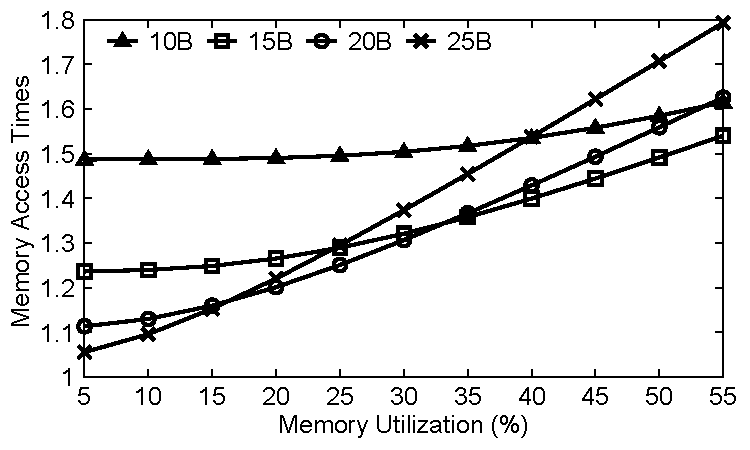
\includegraphics[width=0.6\textwidth]{inline_thresh.pdf}
\caption{Average memory access count under varying inline thresholds (10B, 15B, 20B, 25B) and memory utilizations.}
\label{kvdirect:fig:inline-offline}

\end{figure}

\textit {KV 大小}是指键和值的总大小。
小于阈值的KV在哈希索引中内联(inline)存储,以保存对获取KV数据的额外存储器访问。
内联KV可以跨越多个散列槽,其指针和二级散列字段被重新用于存储KV数据。
内联所有可装入铲斗的KV可能不是最佳选择。
为了最小化平均访问时间,假设可以同等地访问越来越小的密钥,则更希望内联小于\textit {内联阈值}的KV。
为了量化所有桶中使用的桶的部分,我们使用\textit {内存利用率}而不是负载率(load factor),因为它更多地涉及可以适合固定内存量的KV的数量。
如图\ref {kvdirect:fig:inline-offline}所示,对于某个内联阈值,由于更多的哈希冲突,平均内存访问计数随内存利用率的增加而增加。
较高的内联阈值显示内存访问计数的更陡峭的增长曲线,因此可以找到最佳内联阈值以最小化在给定内存利用率下的内存访问。
与哈希索引比率一样,也可以在初始化时配置内联阈值。

当存储桶中的所有插槽都已填满时,有几种解决方案可以解决散列冲突。
Cuckoo哈希\cite {pagh2004cuckoo}和跳房子哈希(Hopscotch Hash)\cite {herlihy2008hopscotch}通过在插入过程中移动占用的插槽来保证恒定时间查找。
但是,在写入密集型工作负载中,高负载率下的内存访问时间会经历大的波动。
线性探测可能受到主群集的影响,因此其性能对散列函数的均匀性敏感。
我们选择\textit {拉链法}来解决哈希冲突,这会平衡查找和插入,同时对哈希群集更加健壮。

%In KV-Direct, we measure memory utilization instead of load factor, because chaining has dynamic size and that we care more about the overall storage efficiency counting all indexing, metadata and memory fragmentation overhead.
%Clearly, small KVs cause lower memory utilization due to metadata overhead.
%The optimal hash index ratio is chosen at initialization time according to workload to balance average access time and memory utilization.

\subsubsection{Slab 内存分配器}
\label{kvdirect:sec:slab}

链式散列槽和非内联KV需要动态内存分配。
我们选择slab内存分配器\cite {bonwick1994slab}来实现每个分配和释放的$O(1)$平均内存访问。主平板分配器逻辑在主机CPU上运行,并通过PCIe与KV处理器通信。
Slab分配器将分配大小四舍五入到最接近的2的幂,称为\textit {slab 大小}。
它为每个可能的slab大小(32,64,\ldots,512字节)和全局 \textit {分配位图}维护\textit {空闲 slab 池},以帮助将小的空闲slab合并回更大的slab。
每个空闲slab池是一个\textit {slab 条目}数组,由一个地址字段和一个slab类型字段组成,表示slab条目的大小。
可以在NIC上缓存可用的slab池。缓存与批量的slab条目中的主机内存同步。通过批处理分摊,每次分配或解除分配需要少于0.07的DMA操作。
当一个小板坯池几乎是空的时,需要拆分较大的板坯。
因为slab类型已经包含在slab条目中,所以在\textit {slab 分割}中,slab条目只是从较大的池复制到较小的池,而不需要计算。
在slab条目中包括slab类型也可以节省通信成本,因为一个slab条目可能包含多个槽。

在重新分配时,slab分配器需要检查释放的slab是否可以与其邻居合并,需要至少一次读取和写入分配位图。
受垃圾收集的启发,我们建议\textit {懒惰 slab 合并}在一个slab池几乎为空时并且没有更大的slab池有足够的slab来拆分时批量合并空闲slab。

\subsubsection{乱序执行引擎}
\label{kvdirect:sec:ooo}

\begin{figure}[t]
\centering
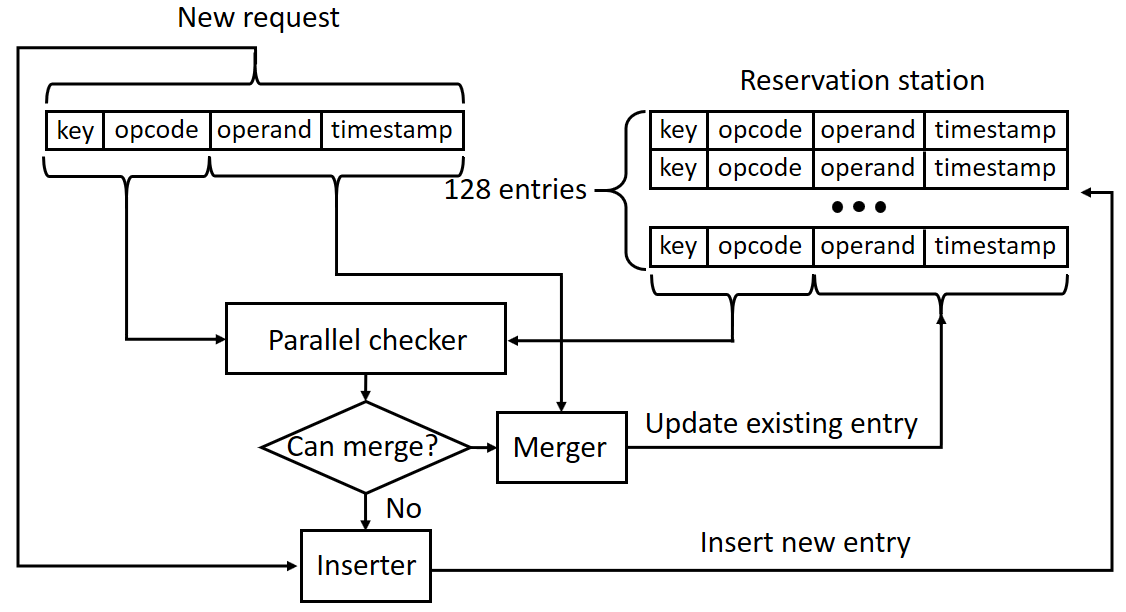
\includegraphics[width=.9\textwidth,page=1]{dynamic_scheduler.PNG}
\caption{乱序执行引擎。}
\label{kvdirect:fig:ooo-mem-access}
\end{figure}

在KV处理器中使用相同密钥的两个KV操作之间的依赖性将导致数据危险和管道停滞。
这个问题在单键原子中被放大,其中所有操作都是依赖的,因此限制了原子的吞吐量。
我们从计算机体系结构借用动态调度的概念,并实现\textit {保留站}(reservation station)来跟踪所有正在进行的KV操作及其\textit {执行上下文}。
为了使PCIe,DRAM和处理流水线饱和,需要多达256个正在执行的KV操作。
但是,并行比较256个16字节密钥将占用FPGA的40%逻辑资源。
相反,我们将KV操作存储在片上BRAM中的小哈希表中,由密钥的哈希索引。
为了简化哈希冲突解决方案,我们认为KV操作具有相同的哈希值,因此可能存在误报,但它永远不会错过依赖关系。
具有相同散列的操作在链中组织并顺序检查。
散列冲突会降低链检查的效率,因此保留站包含1024个散列槽,使哈希冲突可能性低于25%。

保留站不仅保留挂起的操作,还缓存\textit {数据转发}(data forwarding)的最新值。
当主处理流水线完成KV操作时,其结果返回给客户端,最新值被转发到保留站。
逐个检查相同散列槽中的待定操作,并立即执行具有匹配密钥的操作并从保留站移除。
对于原子操作,计算在专用执行引擎中执行。
对于写入操作,将更新缓存的值。
执行结果直接返回给客户端。
在扫描从属操作链之后,如果更新了高速缓存的值,则向主处理管道发出PUT操作以进行高速缓存写回。
这种数据转发和快速执行路径使单键原子能够在每个时钟周期(180~Mops)内处理一次操作,消除了常用密钥在工作负载下的线头阻塞,并确保一致性,因为在同一个密钥上没有两个操作可以在主处理管道中同时进行。


\subsubsection{DRAM 负载分配器}
\label{kvdirect:sec:dram-cache}

\begin{figure}[t]
\centering
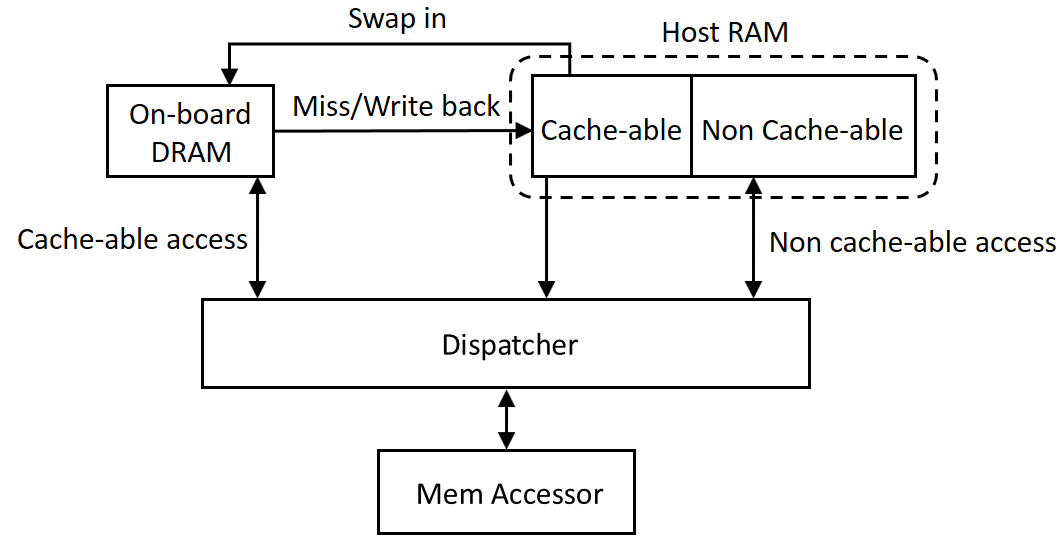
\includegraphics[width=0.8\textwidth,page=1]{load_balancer.PNG}
\caption{DRAM 负载分配器。}
\label{kvdirect:fig:cache}

\end{figure}

为了进一步减轻PCIe的负担,我们在PCIe和NIC板载DRAM之间调度内存访问。
我们的NIC DRAM具有4~GiB大小和12.8~GB / s的吞吐量,比主机DRAM(64~GiB)上的KVS存储小一个数量级,并且比PCIe链路(14~GB / s)稍慢。
一种方法是将固定部分的KVS放入NIC DRAM中。但是,NIC DRAM太小而无法承载大部分内存访问。
另一种方法是使用NIC DRAM作为主机内存的缓存,由于我们的NIC DRAM的吞吐量有限,吞吐量会降低。

我们采用混合解决方案将DRAM用作主机内存中固定部分KVS的缓存,如图\ref {kvdirect:fig:cache}所示。
可缓存部分由存储器地址的散列确定,其粒度为64字节。选择散列函数,使得散列索引和动态分配的存储器中的地址具有可高速缓存的相同可能性。
整个KVS内存中可缓存内存的部分称为\textit {负载分配比例}($ l $)。
使用更大的负载调度比$ l $,将更多负载分配给板载DRAM,并且缓存命中率$ h(l)$将增加。
假设缓存命中率可能是$ h(l)$。
为了平衡PCIe和板载DRAM上的负载,应优化负载调度比$ l $,使得:
$$\frac{l}{tput_{DRAM}} = \frac{(1-l) + l \cdot (1-h(l))}{tput_{PCIe}}$$

特别的,在均匀(uniform)负载下,令 $k$ 是板上 DRAM 大小和主机 KV 存储大小之比,则缓存命中率 $h(l) = \frac{\textnormal{cache size}}{\textnormal{cache-able memory size}} = \frac{k}{l}$,当 $k \leq l$ 时。
一致负载下的缓存并不高效。
在长尾负载(Zipf 分布)下,设 $n$ 是 KV 的总数,则大致上 $h(l) = \frac{\log (\textnormal{缓存大小})}{\log (\textnormal{可缓存部分大小})} = \frac{\log (kn)}{\log (ln)}$,当 $k \leq l$ 时。
在长尾工作负载下,1G语料库中1M缓存的缓存命中可能性高达0.7。
最优的 $l$ 可以得出数值解,将在 \S\ref{kvdirect:sec:different-nic} 中讨论。

\egg{
\subsubsection{Congestion Avoidance}
\label{kvdirect:sec:congestion-avoidance}

In addition to throughput, another important factor is latency.
From the client's perspective, the KV processor is a path with multiple bottlenecks and buffers, \eg, PCIe and DRAM access.
If all buffers in the KV processor are filled up, the GET latency would exceed 10~$\mu$s.
To mitigate the bufferbloat problem, we implement a congestion avoidance logic to limit the number of in-flight KV operations \textit{inside the KV processor}.
The KV processor maintains a \textit{KV operation window} and leverages credit-based flow control mechanism in RDMA to back-pressure KVS clients.
To adapt KV operation window size to the workload, we measure the running average of KV processing delay and adjust the window size according to TCP Vegas congestion avoidance algorithm~\cite{brakmo1995tcp}.
%We use delay as the congestion signal instead of ECN, because the queues whose sizes are hard to measure.
}
